\chapter{Implementation}

In this chapter we will outline the program structure. We will
demonstrate the flexibility as well as the limitations of our
implementation.


%%%%%%%%%%%%%%%%%%%%%%%%%%%%%%%%%%%%%%%%%%%%%%%%%%%%%%%%%%%%%%%%%%%%
%                                                                  %
%                      Structure of the QMC Program                %
%                                                                  %
%%%%%%%%%%%%%%%%%%%%%%%%%%%%%%%%%%%%%%%%%% %%%%%%%%%%%%%%%%%%%%%%%%%
\section{Structure the QMC Program}


%%%%%%%%%%%%%%%%%%%%  Programming Philosophy  %%%%%%%%%%%%%%%%%%%%%%
\subsection{Programming Philosophy}

There are three major concepts concerning the implementation of any
large program:

\begin{enumerate}
  \item{} Speed - the computational time (CPU).
  \item{} Flexibility - ability to handle many different special cases.
  \item{} Readability - how easy it is to understand the program (and
  make modifications).
\end{enumerate}

In order to include flexibility, the
program should consist of many small building blocks, that may easily
be replaced by other similar blocks. The program structure should also
be legible. Often, modifications of existing programs need to be done,
either by the programmers themselves, or by other users. This task may
be very time consuming, especially if the program is difficult to
understand. The algorithms and data structure 
need to be well documented, the building blocks\footnote{Classes
  in C++, modules in Fortan90/50 etc.} should seem like natural
choices, and the variables names should be meaningful. \newline

Futhermore, programs may run for days on powerful machines in order to
accuire the desired result. Therefore, a great deal of effort must be
put into the design and development of the program. \newline


%%%%%%%%%%%%%%%%%%%% Main Program Structure %%%%%%%%%%%%%%%%%%%%%%%
\subsection{Main Program}

Our first concern is to recognice what the program is going to do, and
to form a program stucture. We divide the program into blocks, that
each preform some specific task. Figure \ref{program_stucture} illustrates
the basic structure of our main program. 

\begin{figure}[hbtp]
\begin{center}
  \epsfig{file=Implementation/program.eps, height=8cm}
  \caption{Variational Monte-Carlo program structure}
  \label{program_stucture}
\end{center}
\end{figure}

Generally, the user must provide some input to specify what the
computer is going to calculate.  After the input is specified, the
user does not need to do anything until the program is terminated. The
output should be presented in an easy and orderly fashion; either at
the end of the program execution, or by user specifications after the
run is completed. \newline

Dependent of the user input, the program will execute one or more runs
of the VMC algorithm. The program loops different configurations and
parameter settings, in order to localize an energy (or variance)
minimum. Each setting generate the input, the \emph{initial setup},
for a VMC calulation, and for each VMC run the program genrates an
\emph{output}. Typically, this output is for user deguging. For
example, if the initial parameter input is off bounds (and the program
terminates without finding an energy minimum) the user may chech these
outputs to adjust the user specified input for another run.


%%%%%%%%%%%%%%%%%%%%%%%%% Input Structure %%%%%%%%%%%%%%%%%%%%%%%%%
\subsection{Input}

The input structure is given by figure \ref{input_stucture}.

\begin{figure}[hbtp]
\begin{center}
  \epsfig{file=Implementation/input.eps, height=5.7cm}
  \caption{Input structure}
  \label{input_stucture}
\end{center}
\end{figure}

The user must specify the atom to be studied, and what state is to be
found - e.g. the He 2$^{nd}$ excited $^1S_0$-state. The trial wavefunction
must also be specified, both the variational form of the orbital
wavefuntions and of the Jastrow-factor. These choices gives raise to a
set of parameters, and the user must provide some inital guess, and
tell wich parameters is to be varied. The user must further set some
termination criteria, TC, for example number of Monte-Carlo
cycles. Some other parameters must also be set, either by the program,
or by the user; number of dimensions, output file-name(s), etc.


%%%%%%%%%%%%%%%% Loop Parameters & Configurations %%%%%%%%%%%%%%%%%
\subsection{Loop Parameters \& Configurations}

Figure \ref{loop_parameters_config} outlines the \emph{loop parameters \&
configurations} structure.

\begin{figure}[hbtp]
\begin{center}
  \epsfig{file=Implementation/loop_parameters_config.eps, height=7cm}
  \caption{Structure of parameter and configuration loop}
  \label{loop_parameters_config}
\end{center}
\end{figure}

We want to test different trial wave-function configurations;
i.e. different sets of the orbital wave-functions, and different sets
of Jastrow-factors\footnote{In our program these variations are left
  to the user, i.e. the user may only choose one configuration for
  each run.}.  \newline

For one fixed configuration, a set of variational
parameters, $\{\alpha_i\}$, is to be optimized with respect to either
minimization of energy or variance. We may start with one initial
guess of the set of parameters, $\{\alpha_i\}$, and one TC. When the
TC are met, we may improve our initial guess of parameters, and may
also change the TC. \newline 

For example, we may start with one-hundred thousand
Monte-Carlo cyles, make a local variation of the parameters, and move
our next parameter guess to the energy minimum of that local
variation. When the movement is no longer uni-directional we can
increase the TC to one million cycles, and may also reduce the degree
of variation. In this way, one run of the program may pinpoint
the energy-minimum with quite good accuracy, without too great expense
of computational time.

%%%%%%%%%%%%%%%%%%%%%%%%%% Initial Setup %%%%%%%%%%%%%%%%%%%%%%%%%%
\subsection{Initial Setup}

To begin one VMC run, a complete initial setup must be set; figure
\ref{initial_setup}. 

\begin{figure}[hbtp]
\begin{center}
  \epsfig{file=Implementation/initial_setup.eps, height=7.5cm}
  \caption{Initial setup}
  \label{initial_setup}
\end{center}
\end{figure}

In addition to the choice of trial wave-function, variational
parameters and TC, the program must initialize several parameters and
variables\footnote{These issues will be addressed {\bf
    \emph{later}}. }. Also, initial spatial coordinates of each
particle, and their respective spin, must be set.

The metropolis algorithm, {\bf \emph{described in
    section \ref{metropolis} }}, duplicates the behavior of the
wave-function. Before we begin the VMC sample, we want to make sure
that the particles initial positions are representative with respect
to the wave-function. Therefore, the metropolis algorithm is applied
several times to randomly chosen spatial and spin coordinates; the
coordinates are \emph{thermalized}.


%%%%%%%%%%%%%%%%%%%%%%%%%%%%%% VMC %%%%%%%%%%%%%%%%%%%%%%%%%%%%%%%%
\subsection{VMC}

Figure \ref{vmc} illustrates the basic principles of the different VMC
algorithms; all of which we wish to study in this thesis. 


\begin{figure}[hbtp]
\begin{center}
 % \epsfig{file=Implementation/vmc.eps, height=8.8cm}
  \documentclass{article}

\usepackage[latin1]{inputenc}
\usepackage{tikz}
\usetikzlibrary{shapes,arrows}
\usepackage{verbatim}

\begin{comment}
:Title: Simple flow chart
:Tags: Diagrams

With PGF/TikZ you can draw flow charts with relative ease. This flow chart from [1]_
outlines an algorithm for identifying the parameters of an autonomous underwater vehicle model. 

Note that relative node
placement has been used to avoid placing nodes explicitly. This feature was
introduced in PGF/TikZ >= 1.09.

.. [1] Bossley, K.; Brown, M. & Harris, C. Neurofuzzy identification of an autonomous underwater vehicle `International Journal of Systems Science`, 1999, 30, 901-913 


\end{comment}


\begin{document}
\pagestyle{empty}


% Define block styles

\tikzstyle{decision} = [diamond, draw, fill=blue!20, 
    text width=4.5em, text badly centered, node distance=3cm, inner sep=0pt]
\tikzstyle{block} = [rectangle, draw, fill=blue!20, 
    text width=5em, text centered, rounded corners, minimum height=4em]
\tikzstyle{line} = [draw, -latex'];
\tikzstyle{cloud} = [draw, ellipse,fill=red!20, node distance=3cm,
    minimum height=2em];
    
\begin{tikzpicture}[node distance = 2cm, auto]
    % Place nodes

    \node [block] (init) {initialize};
    \node [cloud, left of=init] (expert) {expert};
    \node [cloud, right of=init] (system) {system};
    \node [block, below of=init] (identify) {identify candidate models};
    \node [block, below of=identify] (evaluate) {evaluate candidate models};
    \node [block, left of=evaluate, node distance=3cm] (update) {update model};
    \node [decision, below of=evaluate] (decide) {is best candidate better?};
    \node [block, below of=decide, node distance=3cm] (stop) {stop};
    % Draw edges
    \path [line] (init) -- (identify);
    \path [line] (identify) -- (evaluate);
    \path [line] (evaluate) -- (decide);
    \path [line] (decide) -| node [near start] {yes} (update);
    \path [line] (update) |- (identify);
    \path [line] (decide) -- node {no}(stop);
    \path [line,dashed] (expert) -- (init);
    \path [line,dashed] (system) -- (init);
    \path [line,dashed] (system) |- (evaluate);
\end{tikzpicture}


\end{document}
  \caption{Three different algorithms for VMC: \newline
  (a) Move all/none particles \newline
  (b) Move one/no particle \newline
  (c) Move some particles}
  \label{vmc}
\end{center}
\end{figure}

In the first algorithm, figure \ref{vmc} (a), either all, or none, of
the particles are moved. This algorithm is easy to implement, but is
the most time-consuming of the three\footnote{Even though it is easy
  to implement, we will optimize our program with respect to the other
  two VMC algorithms. So, this ease is not reflexted in the code
  presented in \emph{?????}.}. In the second algorithm, depicted 
in figure \ref{vmc} (b), we sample the local energy after only one/no
particle is moved. In figure \ref{vmc} (c) we move some particles; 
we move one particle at a time, and conduct induvidual metropolis tests,
before we updating the local energy.

The \emph{Propose move} algorithm is depicted in figure \ref{propose_move}.

\begin{figure}[hbtp]
\begin{center}
  \epsfig{file=Implementation/propose_move.eps, height=3.8cm}
  \caption{Structure of \emph{Propose move}; proposed displacement of
    one particle}
  \label{propose_move}
\end{center}
\end{figure}

The \emph{Spin Flip} algorithm means that the particle may undergo a
spin flip with a randomly chosen particle. If the two particle have
the same spin, nothing happens. If the two particles have
different spin, the spins are exchanged. \newline
Two possible approches for the \emph{Randomize Position} algoritm:

\begin{enumerate}
  \item{}
    Variate position around the particles current location:

    \begin{equation*}
      x_{new}=x_{old}+\text{\small{RANDOM}}
    \end{equation*}

    where RANDOM is a random number based on e.g. a uniform distribution
    or a gaussian distribution.
  \item{}
    Importance Sampling:

    \begin{equation*}
      x_{new}=\Upsilon(\text{\small{RANDOM}})
    \end{equation*}

    where the function $\Upsilon$ duplicate the behaviour of the
    wave-function.
\end{enumerate}




%%%%%%%%%%%%%%%%%%%%%%%%%%%%%%%%%%%%%%%%%%%%%%%%%%%%%%%%%%%%%%%%%%%%%%
%                                                                    %
%                           Data Structure                           %
%                                                                    %
%%%%%%%%%%%%%%%%%%%%%%%%%%%%%%%%%%%%%%%%%%%%%%%%%%%%%%%%%%%%%%%%%%%%%%

\section{Data Structure}

We keep the Slater determinant and correlation wave-function in
separate classes. Let us start out with the correlation. For the
Metropolis step we need the ratio between the new and the old
wave-functions. Furthermore, we need the value of the correlation, and
its first and second derivatives, in order to preform a sample of the
local energy. \newline
We limit our attention to correlations, $G$ equal either $J$ or $e^J$,
where the Jastrow-factor is given by: 

\begin{equation}
  J = \sum_{i=0}^{\bar{N}}\sum_{j > i} f_{ij}
\end{equation}

where $N$ is the number of particles, $\bar{N}=N-1$, and

\begin{equation}
  f_{ij} = f(r_{ij})
\end{equation}

where $r_{ij}$ is the inter-electronic distance between electron $i$
and electron $j$.

Before we give the structure of the correlation, we first establish
classes to keep track of the inter-electronic distances,
\emph{Distance} and \emph{DistanceDiff}, the values of the $f_{ij}$'s,
\emph{Jastrow} and \emph{JastrowDiff}, and the derivatives,
\emph{Derivatives}.




%%%%%%%%%%%%%%%%%%%%% Distance and DistanceDiff %%%%%%%%%%%%%%%%%%%%
\subsection{Distance and DistanceDiff} 

The two classes, \emph{Distance} and \emph{DistanceDiff}, keep track
of the inter-electronic distances.  \newline
For \emph{Distance}, $r_{ij}$ is given by:

\begin{equation}
  r_{ij} = \left[
  \begin{array}{ccccccccc}
    0&r_{01}&r_{02}&\dots & r_{0i} &\dots &\dots & r_{0 \bar{N}} \\
    0&  0   &r_{12}&\dots & r_{1i} &\dots &\dots & r_{1 \bar{N}} \\
    0&  0   &  0   &\ddots& \vdots &\dots &\dots & \vdots       \\
    0&  0   &  0   &0& r_{\bar{i}i}&\dots &\dots & \vdots       \\
    0&  0   &  0   &  0   &  0&r_{ii^{^+}}&\dots & r_{i \bar{N}} \\
    0&  0   &  0   &  0   &   0    &  0   &\ddots& \vdots \\
    0&  0   &  0   &  0   &   0    &  0   & 0    &r_{\bar{\bar{N}} \bar{N}} \\
    0&  0   &  0   &  0   &   0    &  0   & 0    &  0
  \end{array} \right]
\label{r_ij}
\end{equation}

where $\bar{i}=i-1$, $i^{^+}=i+1$, $\bar{N}=N-1$ and
$\bar{\bar{N}}=N-2$. This information is stored in a single array of
length $N\dot(N-1)/2$, 

\begin{equation}
  \begin{array}{ccccc}
  rij =
  &|\underbrace{r_{01}, r_{02}, \dots, r_{0 \bar{N}} }
  &|\underbrace{ r_{12}, \dots, r_{1 \bar{N}} }
  &| \dots &|\underbrace{ r_{\bar{\bar{N}} \bar{N}} }  >\\
  & N-1 & N-2 & & 1\phantom{ii}
  \end{array}
  \label{r_ij_array}
\end{equation}

With a proposed move of electron $i$, only $N-1$ values need to be
updated. These values are stored in 

\begin{equation}
  rij\_new\_column = | r_{0i}, r_{1i}, \dots, r_{\bar{i}i}, r_{ii^{^+}},
  \dots, r_{i \bar{N}} >
\end{equation}

If the move is accepted, the values of \emph{rij\_new\_column} replace the
corresponding values in $rij$.

\emph{Distance} and
\emph{DistanceDiff} are quite similar, except \emph{DistanceDiff}
allows a variation of a coordinate.
For the \emph{DistanceDiff} class, the upper triangular matrix $r_{ij}$
is

\begin{equation}
  r_{ij} = \left[
  \begin{array}{ccccc}
    0 & r_{01}(\xi_1+h) & r_{02}(\xi_2+h)&\dots & r_{0 \bar{N}}(\xi_{\bar{N}}+h) \\
    0 &        0        & r_{12}(\xi_2+h)&\dots & r_{1 \bar{N}}(\xi_{\bar{N}}+h) \\
    0 &        0        &          0            &\ddots &  \vdots       \\
    0 &        0        &          0            &   0   &r_{\bar{\bar{N}} \bar{N}}(\xi_{\bar{N}}+h) \\
    0 &        0        &          0            &   0   &   0  
  \end{array} \right]
\label{r_ij_Diff}
\end{equation}

where $\xi$ is one of the cartesian coordinates. 

\begin{figure}[hbtp]
\begin{center}
  \epsfig{file=Implementation/vector_variation.eps, height=4cm}
  \caption{Addition of a vector at j equals the subtraction of the
  same vector at i}
  \label{vector_variation}
\end{center}
\end{figure}

As be can seen from figure \ref{vector_variation}\footnote{This is
  also easy to see from the relation $r_{ij} = \sqrt{
    \sum_{k=0}^{\bar{d}}(\xi_i^k-\xi_j^k)^2}$, 
where d is the number of dimensions, and $\bar{d}=d-1$.}, 

\begin{equation}
  r_{ij}(\xi_j+h) = r_{ij}(\xi_i-h)
\end{equation}

One object of class \emph{Distance} and 2d objects of class
\emph{DistanceDiff} holds all the information needed of the
inter-electronic distances for numerical calculation of both the
(centered difference) derivative and second derivative. Movement of
one electron consists of $(2d+1)\dot(N-1)$ updates of the distances,
and is thus of order ${\cal O}(N)$. Table \ref{Distance} give a list of the
public algorithms for the classes \emph{Distance} and
\emph{DistanceDiff}.

\begin{table}[hbtp]
\begin{center} {\large \bf Distance and DistanceDiff} \\ 
$\phantom{a}$ \\
\begin{tabular}{ll}
\hline\\ 
{\bf Algorithm}              & {\bf Usage} \\
Distance() or DistanceDiff() &Constructor\\
void attach(...)             &Attach intrinsic properties\\
void initialize()            &Initialize distances\\
void updateProposedMove()    &Calculate new distances for proposed move\\
void acceptMove()            &Accept proposed move\\
void rejectMove()            &Reject proposed move\\
double* getMatrix()          &Returns pointer to $rij$\\
double* getNewColumn()       &Returns pointer to $rij\_new\_column$\\
\hline
\end{tabular} 
\end{center}
\caption{Public algorithms for the classes Distance and DistanceDiff}
\label{Distance}
\end{table}

The differential parameters of
\emph{DistanceDiff}, $h$ and \emph{differentiate}, are assigned to
\emph{DistanceDiff} through the \emph{attach} algorithm. The value $h$
is the value added, or subtracted, to coordinate $differentiate$ of the
trial coordinate. \newline
An example on how to deal with upper triangular matrixes 
is in order. In the \emph{acceptMove} algorithm the new distances of
\emph{rij\_new\_column} is to be put into the upper-triangular matrix
$rij$. Here followes the \emph{acceptMove} algorithm:

{\footnotesize
\begin{enumerate}
\item[]
\begin{verbatim}
void Distance::acceptMove()
{
  __rij = rij-1+currentParticle;
  __rij_new_column = rij_new_column-1;
  int k=numParticles-1;
  for ( int i=0; i<currentParticle; i++ ) {
    (*__rij) = (*++__rij_new_column);
    k--;
    __rij+=k;
  }
  for ( int i=currentParticle+1; i<numParticles; i++)  
    (*++__rij)=(*++__rij_new_column);
  nextParticle();
}
\end{verbatim}

\end{enumerate}
}

For short we set $C=currentParticle$.
The pointer $\_\_rij$ is set to point at $r_{0C}$, if $C\ne
0$\footnote{If $C=0$ $\_\_rij$ is set to point at the element prior
  to the first element of $rij$},  
and $\_\_rij\_new\_column$ is set to point at the element
prior to the first element of $rij\_new\_column$\footnote{We
  create an extra element for this specific purpose.}.
Then we loop $i=0,C-1$, and set the value of $\_\_rij$ equal to the value
of the incremented $\_\_rij\_new\_column$, i.e. $r_{0C}$. We proceed
until $r_{\bar{C}C}$ (where $\bar{C}=C-1$). The pointer
$\_\_rij$ now points at $r_{\bar{C}\bar{N}}$, and in the
second loop it is incremented to point at $r_{CC^{^+}}$ (where $C^{^+}=C+1$),
and so is $\_\_rij\_new\_column$. Both pointers are incremented until
all the values are set, and we finally jump to the next particle.
\newline
Let us give an example of the $\_\_rij\_new\_column$ pointer. For $N=5$
and $C=2$ we have

\begin{equation}
  \begin{array}{cccccc}
  rij =
  |r_{01}, &r_{02}, \phantom{A} r_{03}, \phantom{A} r_{04}, &r_{12},
  \phantom{A} r_{13}, &r_{14}, &r_{23},
  &r_{24}, \phantom{A} r_{34}> \\
  pointer& \Uparrow \phantom{AAAAAAA}& \Uparrow \phantom{AAA}& \uparrow &
  \Uparrow & \Uparrow \phantom{AAAA}\\
  k& \phantom{AAA}3 & \phantom{AAAA}2 & \phantom{aa}1 & \phantom{aa}1 & 
  \end{array}
  \label{r_ij_array}
\end{equation}

We assign values at $\Uparrow$, and the $\uparrow$ is a temporary
pointer between the two loops.
This can more readily be seen by
looking at the corresponding matrix.

\begin{equation}
  r_{ij} = \left[
  \begin{array}{ccccc}
    0 & r_{01} & r_{02} & r_{03}  & r_{04}\\
    0 &   0    & r_{12} & r_{13}  & r_{14}\\
    0 &   0    &   0    & r_{23}  & r_{24}\\
    0 &   0    &   0    &   0     & r_{34}\\
    0 &   0    &   0    &   0     &   0   \\
  \end{array} \right]
\end{equation}

In the first loop we add one less than the number of none-zero
elements in the row we are at. Disregarding the none-zero elements,
this will take us to the element of the next row, with the same last index
(unless we are at the first element, in which case it will take us
to the last element).





%%%%%%%%%%%%%%%%%%%%% Jastrow and JastrowDiff %%%%%%%%%%%%%%%%%%%%
\subsection{Jastrow and JastrowDiff}

The classes \emph{Jastrow} and \emph{JastrowDiff} are similar to
\emph{Distance} and \emph{DistanceDiff}, respectively. First, they
contain information about the $f_{ij}$, in $f\_matrix$ (and the new
values for a proposed move, in \emph{f\_new\_column}). 
Furthermore, \emph{Jastrow} contains information about
the \emph{jastrowian}, $J$, and $\Delta J=J_{new}-J_{old}$.
Updating the $f_{ij}$'s for the jastrowian and its first and second
derivatives is also of order ${cal O}(N)$ (for the movement of one
electron).
Table \ref{Jastrow} lists the public algorithms of \emph{Jastrow} and
\emph{JastrowDiff}.

\begin{table}[hbtp]
\begin{center} {\large \bf Jastrow and JastrowDiff} \\ 
$\phantom{a}$ \\
\begin{tabular}{ll}
\hline\\ 
{\bf Algorithm}                        & {\bf Usage} \\
Jastrow() or JastrowDiff()             &  Constructor\\
void attach(...)                       &  Attach intrinsic properties\\
void initialize()                      &  Initialize the $f_{ij}$'s (and the jastrowian)\\
void updateProposedMove()              &Calculate new $f_{ij}$'s for proposed move\\
void acceptMove()                      &Accept proposed move\\
void rejectMove()                      &Reject proposed move\\
double* getFMatrix()                   &Returns pointer to $f\_matrix$\\
double* getFNewColumn()                &Returns pointer to $f\_new\_column$\\
void getFColumn(int i, double* fColumn)&Returns column i of $f\_matrix$ in fColumn\\
{\bf Jastrow-specific algorithms}      &\\
double\& operator()()                  &Returns the jastrowian, $J$\\
double getDifference()                 &Returns the difference, $\Delta J=J_{new}-J_{old}$\\
\hline
\end{tabular} 
 \end{center}
  \caption{Public algorithms for the classes Jastrow and JastrowDiff}
\label{Jastrow}
\end{table}

For example \emph{getFNewColumn} returns a pointer to:

\begin{equation}
  f\_new\_column = | f_{0i}, f_{1i}, \dots, f_{\bar{i}i}, f_{ii^{^+}},
  \dots, f_{i \bar{N}} >
\end{equation}

where $i$ is the current particle being moved.





%%%%%%%%%%%%%%%%%%%%% Derivatives %%%%%%%%%%%%%%%%%%%%
\subsection{Derivatives}

\emph{Derivatives} manages the derivatives of the $f_{ij}$'s. 
\newline
It is sufficient to calculate either $\frac{\delta f_{ij}}{\delta
  \xi_i}$ or $\frac{\delta f_{ij}}{\delta \xi_j}$, since 

\begin{equation}
  \frac{\delta f_{ij}}{\delta \xi_i} = \frac{\delta r_{ij}}{\delta \xi_i}
  \frac{d f_{ij}} {d r_{ij}} = - \frac{\delta r_{ij}}{\delta \xi_j}
  \frac{d f_{ij}} {d r_{ij}} = - \frac{\delta f_{ij}}{\delta \xi_j}
\end{equation}

In the above calculation we have used

\begin{equation}
  \frac{\delta r_{ij}}{\delta \xi_i^m} = \frac{\delta}{\delta \xi_i^m} 
  \sqrt{ \sum_{k=0}^{\bar{d}} (\xi_i^k-\xi_j^k)^2} =
  \frac{\xi_i^m-\xi_j^m}{r_{ij}} = - \frac{\delta
  r_{ij}}{\delta \xi_j^m} 
\end{equation}

where $\xi_i^m$ is cordinate $m$ of particle $i$, and $\bar{d}=d-1$. \newline
The upper triangular matrix:

\begin{equation}
  \frac{\delta f}{\delta \xi} = \left[
  \begin{array}{ccccc}
    0 & \frac{\delta f_{01}}{\delta \xi_1} & \frac{\delta
    f_{02}}{\delta \xi_2} & \dots & \frac{\delta f_{0\bar{N}}}{\delta
    \xi_{\bar{N}}} \\ 
    0 &        0        & \frac{\delta f_{12}}{\delta \xi_2} & \dots & 
    \frac{\delta f_{1\bar{N}}}{\delta \xi_{\bar{N}}} \\
    0 &        0        &          0            &\ddots &  \vdots       \\
    0 &        0        &          0            &   0   &
    \frac{\delta f_{\bar{\bar{N}}\bar{N}}}{\delta \xi_{\bar{N}}} \\
    0 &        0        &          0            &   0   &   0  
  \end{array} \right]
\label{df_dxi}
\end{equation}

is stored as an array, \emph{derivatives}, similar to that of
eq. (\ref{r_ij_array}). Also, we store 
the upper-triangular matrix of the second derivatives. The calculation
of the first derivative,

\begin{equation}
  \frac{\delta f_{ij}}{\delta \xi_i} \approx \frac{f_{ij}(\xi_i+h) -
  f_{ij}(\xi_i-h)}{2h} 
\end{equation}

and the second derivative,

\begin{equation}
  \frac{\delta^2 f_{ij}}{\delta \xi_i^2} \approx \frac{f_{ij}(\xi_i+h)
  + f_{ij}(\xi_i-h) - 2 f_{ij}}{h^2}
\end{equation}

uses the $f_{ij}$'s updated in \emph{Jastrow} and
\emph{JastrowDiff}. Movement of one particle involves
calculation of $N-1$ values of both $\frac{\delta f_{ij}}{\delta \xi_i}$
and $\frac{\delta^2 f_{ij}}{\delta \xi_i^2}$. Table \ref{Derivatives}
lists the public algorithms of \emph{Derivatives}.

\begin{table}[hbtp]
\begin{center} {\large \bf Derivatives} \\ 
$\phantom{a}$ \\
\begin{tabular}{ll}
\hline\\ 
{\bf Algorithm}                   & {\bf Usage} \\
Derivatives()                     &Constructor\\
void attach(...)                  &Attach intrinsic properties\\
void initialize()                 &Initialize the derivatives\\
void updateDerivatives()          &Calculate the new derivatives for a move\\ 
void acceptDerivatives()          &Updates the 1. and 2. derivatives matrix\\
void rejectDerivatives()          &Jumps to next particle without doing
anything\\
void getDColumn(int i, double* Column) 
  &Returns column i of $\frac{\delta f}{\delta \xi}$ in Column\\
double* getDNewColumn() &Returns pointer to new derivatives\\
void getD2Column(int i, double* Column)
  &Returns column i of $\frac{\delta^2 f}{\delta \xi^2}$ in Column\\
double* getD2NewColumn()&Returns pointer to new second derivatives\\
\hline
\end{tabular} 
 \end{center}
  \caption{Public algorithms for the class Derivatives}
\label{Derivatives}
\end{table}



%%%%%%%%%%%%%%%%%%%%% Correlation %%%%%%%%%%%%%%%%%%%%
\subsection{Correlation}

Before we proceed with the class structure, some theory must be
established. Let us start with the ratio
$\frac{G_{new}}{G_{old}}$, for the Metropolis algorithm. For $G=J$ we
have 

\begin{equation}
  \frac{G_{new}}{G_{old}} = \frac{J_{old}+\Delta J}{J_{old}}
\end{equation}

and for $G=e^J$,

\begin{equation}
  \frac{G_{new}}{G_{old}} = e^{\Delta J}
\end{equation}

$\nabla^2 J$ given by, 

\begin{equation}
  \nabla^2 J = \sum_{i=0}^{\bar{N}} \nabla_i^2 J =
  \sum_{i=0}^{\bar{N}} \nabla_i^2 \sum_{k<l} f_{kl} = 
  \sum_{i=0}^{\bar{N}} \left[ \sum_{k<l} \delta_{li} \nabla_i^2 f_{kl}
  + \sum_{k<l} \delta_{ki} \nabla_i^2 f_{kl} \right]
\end{equation}

where $\nabla_i^2 f_{ij} = \sum_{k=0}^{\bar{d}} \frac{\delta^2
  f_{ij}}{(\delta \xi_i^k)^2}$, and $\delta_{li}$ is the
Kronecker-delta. We define

\begin{equation}
  \nabla_i^2 J \equiv \sum_{j=0}^{i-1} \nabla_i^2 f_{ij}  +
  \sum_{j=i+1}^{\bar{N}} \nabla_j^2 f_{ij}
\end{equation}

and get 

\begin{equation}
  \nabla^2 J = \sum_{i=0}^{\bar{N}} \left[ \sum_{j=0}^{i-1} \nabla_i^2 f_{ij}
  + \sum_{j=i+1}^{\bar{N}} \nabla_i^2 f_{ij} \right] =
  \sum_{i=0}^{\bar{N}} \nabla_i^2 J
\end{equation}

from the relation $\nabla_i^2 f_{ij} = \nabla_j^2 f_{ij}$. If we move
one particle, $C$, all values in $\nabla^2_C J$, and one of the values
in $\nabla^2_i J$, $i\ne C$, are changed;

\begin{equation}
  \nabla_i^2 J^{new} = \nabla_i^2 J^{old} + \nabla_i^2 f_{iC}^{new} - \nabla_i^2 f_{iC}^{old}
\end{equation}

for all $i\ne C$, and

\begin{equation}
  \nabla_C^2 J^{new} = \sum_{i \ne C} \nabla_i^2 f_{iC}^{new}
\end{equation}

By changing only these values, we have an algorithm of order ${\cal O}(N)$
for the update of $\nabla^2 J$. \newline
For $\nabla J$, we have

\begin{equation}
  \nabla J = \left| \frac{\delta J}{\delta \xi_0^0},
  \dots , \frac{\delta J}{\delta \xi_{\bar{d}}^0}, \dots,
  \frac{\delta J}{\delta \xi_0^{\bar{N}}}, \dots, \frac{\delta J}{\delta
  \xi_{\bar{d}}^{\bar{N}}} \right>
\end{equation}

where

\begin{equation}
  \frac{\delta J}{\delta \xi^i} = \frac{\delta}{\delta \xi^i}
  \sum_{k<l} f_{kl} = \sum_{j=0}^{i-1} \frac{\delta f_{ji}}{\delta
  \xi^i}  + \sum_{j=i+1}^{\bar{N}} \frac{\delta f_{ij}}{\delta \xi^i} 
  = \sum_{j=0}^{i-1} \frac{\delta f_{ji}}{\delta
  \xi^i}  - \sum_{j=i+1}^{\bar{N}} \frac{\delta f_{ij}}{\delta \xi^j}
\end{equation}

since $\frac{\delta f_{ij}}{\delta \xi^i} = - \frac{\delta
  f_{ij}}{\delta \xi^j}$. 
All the values of the derivatives are kept
in the $d$ objects of class \emph{Derivatives}, and its easy to
calculate the above expression. However, we wish to keep the order of
our correlation routines as low as possible, so we follow a procedure
similar to that of $\nabla^2 J$;

\begin{equation}
  \frac{\delta J^{new}}{\delta \xi^i} = \frac{\delta J^{old}}{\delta
  \xi^i} + \frac{\delta f_{ji}^{new}}{\delta \xi^i} - \frac{\delta
  f_{ji}^{old}}{\delta \xi^i} 
\end{equation} 

for $i<C$,

\begin{equation}
  \frac{\delta J^{new}}{\delta \xi^i} = \frac{\delta J^{old}}{\delta
  \xi^i} - \frac{\delta f_{ji}^{new}}{\delta \xi^j} + \frac{\delta
  f_{ji}^{old}}{\delta \xi^j} 
\end{equation} 

for $i>C$, and for $C$

\begin{equation}
  \frac{\delta J^{new}}{\delta \xi^C} 
  = \sum_{j=0}^{C-1} \frac{\delta f_{jC}^{new}}{\delta
  \xi^C}  - \sum_{j=C+1}^{\bar{N}} \frac{\delta f_{Cj}^{new}}{\delta \xi^j}
\end{equation}

For $G=J$ we can use the above relations directly. For $G=e^J$ a few
minor modifications must be made:

\begin{equation}
  \nabla e^J = \nabla J \dot e^J
\end{equation}

and

\begin{equation}
  \nabla^2 e^J = \nabla (\nabla J \dot e^J) = \left[ \nabla^2 J +
  (\nabla J)^2  \right] e^J
\end{equation}

I.e. $e^J$, $\nabla J$ and $\nabla^2 J$ holds all the information needed to
compute $\nabla e^J$ and $\nabla^2 e^J$. The above computations are
also of the order ${\cal O}(N)$. \newline


\emph{Correlation} is the class used by the VMC-algorithm to manage
all information 
about the correlation. It is used to calculate the gradient, and the
gradient squared, of the correlation. Also, the ratio
$\frac{G_{new}}{G_{old}}$ for a proposed move is calculated, as well
as the value of the correlation, $G$, itself. Routines for both
thermalization- and VMC-moves are implemented. \newline
Table \ref{Correlation} lists the public algorithms of \emph{Correlation}.

\begin{table}[hbtp]
\begin{center} {\large \bf Correlation} \\ 
$\phantom{a}$ \\
\begin{tabular}{ll}
\hline\\ 
{\bf Algorithm}                 & {\bf Usage} \\
Derivatives(Domain\& domain)    &Constructor\\
void proposeMove()              &Updates the values (in the Jastrow and
Distance objects)\\
 & needed to determine the ratio $\frac{G_{new}}{G_{old}}$\\
void initializeThermalizedMove()&Initializes the Jastrow and Distance objects\\
void acceptThermalizedMove()    &Updates the Jastrow and Distance objects\\
void rejectThermalizedMove()    &Jumps to next particle without doing anything\\
void initializeVMC()            &Initializes the JastrowDiff, DistanceDiff 
              and Derivatives\\ 
&objects, and initializes $\nabla G$ and $\nabla^2 G$\\
void acceptVMCMove()            &Update $\nabla G$ and $\nabla^2 G$,
and updates the Jastrow, JastrowDiff,\\
& Distance, DistanceDiff and Derivatives objects\\
void rejectVMCMove()            &Jumps to next particle without doing anything\\
double operator()()             &Returns the correlation, $G$,
i.e. either $J$ or $e^J$\\
double getRatio()               &Returns the ratio $\frac{G_{new}}{G_{old}}$\\
double* getGradient()           &Returns pointer to $\nabla G$\\
double getGrad2()               &Returns the value of $\nabla^2 G$\\
\hline
\end{tabular} 
 \end{center}
  \caption{Public algorithms for the class Correlation}
\label{Correlation}
\end{table}

The constructor uses the \emph{Domain} class to access information
about properties like the number of particles $N$, the number of
dimensions $d$, and all the coordinates. The \emph{proposeMove}
algorithm updates the changes in the jastrowian due to a proposed move
in the trial coordinate. Furthermore, it stores the
new inter-electronic distances, and the new $f_{ij}$'s in two arrays;
\emph{rij\_new\_column} in the object of class\emph{Distance} and
\emph{f\_new\_column} in the object of class \emph{Jastrow}. \newline 
If the move is accepted, the values of the differences must be
updated, as well as the derivatives and the gradients (for a VMC
move\footnote{In the case of thermalization, no
  sample of the energy is preformed, so no derivatives (or
  differences) are calculated.}). 
In the \emph{acceptVMCmove} algorithm, see table \ref{Correlation}, the
values of $\nabla J$ and $\nabla^2 J$ are calculated. $\nabla G$
and $\nabla^2 G$ are not calculated until the \emph{getGradient} and
\emph{getGrad2} routines.
Finally, all new values must be assigned to their respective
upper-triangular matrices, before we proceed to the next particle. 
\newline
If the move is not accepted, we simply proceed to the next particle,
without performing any changes.



%%%%%%%%%%%%%%%%%%%%% CoorExt %%%%%%%%%%%%%%%%%%%%
\subsection{CoorExt}

The class \emph{CoorExt}, defined in \emph{Coor.h}, manages the
particles coordinates. Table 
\ref{CoorExt} lists the public algorithms of \emph{CoorExt}. 

\begin{table}[hbtp]
\begin{center} {\large \bf CoorExt} \\ 
$\phantom{a}$ \\
\begin{tabular}{ll}
\hline\\ 
{\bf Algorithm}                   & {\bf Usage} \\
CoorExt()                         & Empty constructor\\
CoorExt(double* x, int \_len,     & Constructor\\
\phantom{a} int \_\_spin, double* \_ext)& \\
void attach(double* \_\_x, int \_len,& Attaches intrinsic properties\\
\phantom{a} int \_\_spin, double* \_ext)& \\
double\& operator()()             & Returns the current cartesian coordinate\\
double\& operator()(int num)      & Returns coordinate num\\
void operator++(int)              & Increments pointer to next cartesian coordinate\\
void resetPtr                     & Resets pointer to first cartesian coordinate\\
int getLen()                      & Returns the number of cartesian coordinates\\
double r()                        & Returns the distance form the nucleus\\
void calculateR()                 & Computes the distance to the nucleus\\
int\& spin()                      & Returns the electron eigen-spin\\
int flipSpin()                    & Returns negative multiple of spin\\
double param(int i)               & Returns the value of parmeter number i; ext[i]\\
\hline
\end{tabular} 
 \end{center}
  \caption{Public algorithms for the class CoorExt}
\label{CoorExt}
\end{table}

\emph{CoorExt} contains all the information needed of each electron;
its cartesian coordinates and its eigen-spin. Furthermore, it contains
a pointer to the variational parameters of the Slater determinant
orbital wave-functions. In this manner one orbital function may be
computed directly given one \emph{CoorExt} object.
Also, the electron distance from the origin is calculated, and it
allows a spin flip.



%%%%%%%%%%%%%%%%%%%%% FuncSetMultivar %%%%%%%%%%%%%%%%%%%%
\subsection{FuncSetMultivar}

The class \emph{FuncSetMultivar}, defined in \emph{Func.h}, manages a
set of functions and their 
derivatives. Each column in a Slater matrix is represented as one such
object. Table \ref{FuncSetMultivar} lists some\footnote{All the
  \emph{attach} procedures are left out, Furthermore, most of the
  algorithms are implemented twice; ($\dots$) means either with or
  without an input (\emph{Param\& \_coordinate}).} of the public algorithms
of \emph{FuncSetMultivar}.

\begin{table}[hbtp]
\begin{center} {\large \bf FuncSetMultivar} \\ 
$\phantom{a}$ \\
\begin{tabular}{ll}
\hline\\ 
{\bf Algorithm}                   & {\bf Usage} \\
FuncSetMultivar($\dots$)          & Constructor\\
void init($\dots$)                & Initialize intrinsic properties\\
void calcValueCenter($\dots$)     & Calculates the function values (given coordinate)\\
void calcValueSides($\dots$)      & Calculates the function values (given differentiated coordinate)\\

double valuePt()                  & Returns pointer to different calculated values\\
double diff()                     & Calculates the first derivatives\\
double diff(int v)                & Calculates the first derivatives
with respect to the\\
                                  & indexed variable (of all functions)\\
double ddiff()                    & Calculates the second derivatives\\
\hline
\end{tabular} 
 \end{center}
  \caption{Public algorithms for the class FuncSetMultivar}
\label{FuncSetMultivar}
\end{table}

In order to find the derivatives of the functions for a given
coordinate, \emph{calcValueCenter} and \emph{calcValueSides}
must be called prior to \emph{diff}. The second derivatives are
calculated with a call to the \emph{ddiff} algorithm.



%%%%%%%%%%%%%%%%%%%%% Functor %%%%%%%%%%%%%%%%%%%%
\subsection{Functor}

The template class \emph{Functor} defines a functor. 
We have chosen to use a functor-type object, to increase
flexibility, and have the ability to use more complex functions
later without changing too much code\footnote{This is good programming
  philosophy; we may want to improve the program at a later stage.}.
Table \ref{Functor} lists the public algorithm of \emph{Functor}.

\begin{table}[hbtp]
\begin{center} {\large \bf Functor} \\ 
$\phantom{a}$ \\
\begin{tabular}{ll}
\hline\\ 
{\bf Algorithm}                   & {\bf Usage} \\
Functor()                         & Empty constructor\\
Functor(Function\& \_function)    & Constructor\\
void attach(Function\& \_function)& Attaches a function\\
Return operator()(Param\& coor)   & Returns an object of type Return\\
\hline
\end{tabular} 
 \end{center}
  \caption{Public algorithms for the class Functor}
\label{Functor}
\end{table}


Given an argument 
\emph{Param} the functor returns \emph{Return}. Both \emph{Param} and
\emph{Return} are classes, e.g. \emph{double}, \emph{CoorExt} etc.
To give an example, we can create a functor with the call:

{\footnotesize
\begin{enumerate}
\item[]
  \begin{verbatim}
Functor<CoorExt, double>* function;
function = new Functor<CoorExt, double>();
\end{verbatim}

\end{enumerate}
}

We need some formula for calculating the return value of type
\emph{double}, given an object of class \emph{CoorExt}. If we first
define the function \emph{hydr1s} given by:

{\footnotesize
\begin{enumerate}
\item[]
  \begin{verbatim}
double hydr1s(CoorExt& coordinate) {
  return exp(- coordinate.param(0) * coordinate.r());
}
\end{verbatim}

\end{enumerate}
}

and then attach it to the \emph{Functor} object \emph{function}:

{\footnotesize
\begin{enumerate}
\item[]
  \begin{verbatim}
function[0].attach(hydr1s);
\end{verbatim}

\end{enumerate}
}

We may then calculate the value of the function with the call:

{\footnotesize
\begin{enumerate}
\item[]
  \begin{verbatim}
function_value = (function[0])(coordinate);
\end{verbatim}

\end{enumerate}
}

where \emph{coordinate} is an object of class \emph{CoorExt}. 



%%%%%%%%%%%%%%%%%%%%% Random %%%%%%%%%%%%%%%%%%%%
\subsection{Random}

The two classes \emph{Ran0} and \emph{Ran1}, in
\emph{Random.h}, defines the random generators used by the
Metropolis random movement. We want our electrons to move \emph{randomly}
in space, and at the same time we want to reduce the CPU-time of our
calculations. Therefore, the program should be tested with different
random generators. Table \ref{Random} lists the
public algorithms of the random generators.

\begin{table}[hbtp]
\begin{center} {\large \bf Random} \\ 
$\phantom{a}$ \\
\begin{tabular}{ll}
\hline\\ 
{\bf Algorithm}                   & {\bf Usage} \\
Ran0(long seed) or Ran1(long seed)& Constructor\\
double getNum(void)               & Returns double in the range (0,1]\\
\hline
\end{tabular} 
 \end{center}
  \caption{Public algorithms for the class Random}
\label{Random}
\end{table}

We will not get into the details of the random generators, and simply
refere to \emph{???reference here???}. However, of importance to the
user is the integral seed. This seed is changed with each call to
\emph{getNum}. Giving the same seed twice produces the exact same
number, and if called several times they will produce the same
sequences of numbers. To produce indepentent runs, the seed
must differ with each run\footnote{An other problem may also
  arise. Even with two different seeds, one of the sequences may by
  chance produce the other seed, and thereby produce the same sequence
following this number. This problem will not be addressed in this
scope, but note that this chance is extremely small, and given two
different starting positions, the Metropolis algorithm should not
become too biased even if this were to occur.}










































